

\documentclass[11pt]{article}

\ExplSyntaxOn % providing \expandableinput
\cs_new:Npn \expandableinput #1
  { \use:c { @@input } { \file_full_name:n {#1} } }
\ExplSyntaxOff

\usepackage{amsmath,amsthm,amssymb, pdfpages,mathtools}
\usepackage{color}
\usepackage{array}
\usepackage{gastex}
\usepackage{subfigure}
\usepackage[normalem]{ulem}
\usepackage{xcolor,psfrag,graphicx}
\usepackage{setspace}
\usepackage{natbib}
\usepackage{lscape}
\usepackage{enumerate}
\usepackage{appendix}
\usepackage[hidelinks, hypertexnames=false]{hyperref}
\usepackage{lscape}
\usepackage{tabularx}
\usepackage{threeparttable}
\usepackage{caption}
\usepackage{booktabs}
\usepackage{longtable}
\usepackage{fullpage}
\usepackage{url}
\usepackage{setspace}
\usepackage{mathpazo}
\usepackage{rotating}
\usepackage{titlesec}
\usepackage{mdwlist}
\usepackage{paralist}
\usepackage{IEEEtrantools}  	% replacing arrays and tables
\usepackage{CJKutf8}  		% display Chinese
\usepackage{epigraph}
\usepackage{environ}
\usepackage{dsfont}
\usepackage{afterpage}
\usepackage[pagewise]{lineno}
\usepackage{xurl}

\usepackage{multirow}					% Create rows in tables that span multiple columns
\usepackage{dcolumn}
\usepackage{tabularx}
\usepackage{float}
\usepackage[T1]{fontenc}
\usepackage{makecell}
\usepackage{rotating}
\usepackage{lscape}



\setcounter{MaxMatrixCols}{10}

\setlength{\evensidemargin}{0.0in}
 \setlength{\oddsidemargin}{0.0in}
 \setlength{\textwidth}{6.5in}
 \topmargin -0.25in
 \textheight 8.5in
 \hfuzz=50pt
 \pagestyle{plain}
\newcommand{\eqthreshn}{{t^*_N}}
\newcommand{\pnd}{1-p+pF(\eqthreshn)}
\newcommand{\ppnd}{\big(1-p+pF(\eqthreshn)\big)}
\newcommand{\eqmfreq}{{\omega^*}}
\newcommand{\eqmfreqn}{{\omega^*_N}}
\newcommand{\eqmfreqnp}{{\omega^*_{N+1}}}
\newcommand{\eqthresh}{{t^*}}
\newcommand{\eqthreshX}{{t^{**}}}
\newcommand{\nbar}{{\overline{N}}}
\newcommand{\wlim}{\omega_\infty}
\newcommand{\wdye}{\hat{\omega}}
\newcommand{\tdye}{\hat{t}}
\newcommand{\limn}{\lim_{N\to\infty}}
\newcommand{\fsn}{\omega_N^*}
\newcommand{\eqprize}{\phi^*}
\newcommand{\moprize}{\phi^M}
\newcommand{\dif}{\;\mathrm{d}}
\newcommand{\diffp}[2]{\frac{\partial #1}{\partial #2}}
\newcommand{\diff}[2]{\frac{\dif #1}{\dif #2}}
\renewcommand{\Re}{\mathbb{R}}                             
\def\endproof{{\quad}$\blacksquare$}
\newcommand{\indicator}[1]{\mathbbm{1}_{\left[ {#1} \right]}}
\newtheorem{theorem}{Theorem}
\newtheorem{proposition}{Proposition}
\newtheorem{prop}{Proposition}
\newtheorem{example}{Example}
\newtheorem{assumption}{Assumption}
\newtheorem{corollary}[theorem]{Corollary}
\newtheorem{acknowledgement}[theorem]{Acknowledgement}
\newtheorem{definition}{Definition}
\newtheorem{lemma}{Lemma}
\newtheorem{remark}{Remark}
\newtheorem{condition}[theorem]{Condition}
 \setlength{\evensidemargin}{0.0in}
 \setlength{\oddsidemargin}{0.0in}
 \setlength{\textwidth}{6.5in}
 \topmargin -0.25in
 \textheight 8.5in
 \hfuzz=50pt
 \pagestyle{plain}
\newcommand{\Change}[1]{{\color{red}#1}}
\renewcommand{\theenumi}{\roman{enumi}}            
\renewcommand{\labelenumi}{(\theenumi)}

%%%%%%%%%%%%%%%
% Page Format %
%%%%%%%%%%%%%%%
 \setlength{\evensidemargin}{0.0in}
 \setlength{\oddsidemargin}{0.0in}
 \setlength{\textwidth}{6.5in}
 \topmargin -0.25in
 \textheight 8.5in
 \hfuzz=50pt
 \pagestyle{plain}





\begin{document}
{\vspace{-5ex}}
\title{\textbf{Seeing is Believing: Identity, Inequality, and the Impact of Television on the Hispanic Achievement Gap}%Unravel}
\thanks{Many appreciated suggestions, critiques and encouragement were provided by Leonardo Bursztyn, Albert Chen, Lucas Cusimano, Andrés de Loera-Brust, Benjamin Enke, Victor Lima, Aakaash Rao, Jaya Wen, David Yang, and Kotaro Yoshida, seminar participants at EPoD, Harvard PE, and the University of Chicago Honors Thesis Workshop as well as Mark Colombo for technical advice on televisions. This is a condensed, 10 page version of the paper. The full version of this paper can be accessed at \url{https://andrew-kao.github.io/files/sltv_draft.pdf}}\\
}



\author{Andrew Kao\thanks{Harvard University. Email: \texttt{andrewkao@fas.harvard.edu}} }

%\begin{center}
\date{November 2021}
{\vspace{-5ex}}
%\end{center}


\maketitle
{\vspace{-5ex}}
\begin{abstract}
\noindent Hispanics face the lowest high school and college completion rates out of all major ethnic and racial groups in the United States. In this paper, I investigate the impact of Spanish Language Television (SLTV) on Hispanic students in public schools using a spatial regression discontinuity arising from FCC regulation. I find that SLTV improves academic outcomes and narrows the Hispanic achievement gap, increasing SAT and ACT tests taken, enrollment in calculus, and AP exams passed. However, SLTV also causes more Hispanic students to be labelled `limited English proficiency' and bullied on the basis of their ethnicity. I dig into the mechanism driving these contradictory results and find that Hispanic students perform better academically where SLTV programming focuses more on the Hispanic identity, but not when it focus more on role models or education itself. Furthermore, Hispanics with access to SLTV visit Hispanic branded establishments more frequently. Collectively, these findings suggest that the effects of SLTV are driven by its effects on identity.\\\\  % think more about this last sentence!
% \noindent  Can identity reduce inequality? Using a spatial regression discontinuity arising from FCC regulation, I investigate the impact of Spanish Language Television (SLTV) on Hispanic students in public schools. I find that SLTV improves academic performance and helps close the Hispanic achievement gap, increasing SAT and ACT tests taken, enrollment in calculus, and AP exams passed. However, SLTV also causes more Hispanic students to be labelled `limited English proficiency' and bullied on the basis of their ethnicity. I dig into the mechanism driving these results and find that Hispanic students perform better academically where SLTV programming focuses more on the Hispanic identity, but not when they focus more on role models or education itself. Hispanics with access to SLTV also more frequently visit Hispanic branded establishments. Collectively, these findings suggest that identity is a mechanism through which SLTV reduces the Hispanic achievement gap.\\\\
% \noindent  Can identity reduce inequality? Using a spatial regression discontinuity arising from FCC regulation, I investigate the impact of Spanish Language Television (SLTV) on Hispanic students in public schools. I find that SLTV improves academic performance and helps close the Hispanic achievement gap, increasing SAT and ACT tests taken, enrollment in calculus, and AP exams passed. I marshal three sources of evidence that each indicate an identity mechanism is at play: (1) more Hispanic students are labelled `limited English proficiency' and bullied on the basis of their ethnicity in SLTV schools, (2) Hispanic students perform better academically where SLTV programming focuses more on the Hispanic identity, and (3) Hispanics with access to SLTV differentially visit Hispanic branded establishments more frequently. Collectively, they suggest that identity is a mechanism through which SLTV reduces the Hispanic achievement gap.\\\\
\textbf{JEL Codes:} I24, J15, L82, Z13.\\
\textbf{Keywords:} Hispanic, television, education, identity
\end{abstract}




\newsavebox{\tablebox} \newlength{\tableboxwidth}

\setlength{\baselineskip}{22pt}

\renewcommand{\thefootnote}{\fnsymbol{footnote}}


\thispagestyle{empty}

\renewcommand{\thefootnote}{\arabic{footnote}}



\onehalfspacing

%\tableofcontents
\section{Introduction}

\small

%\begin{quotation}
%\textit{[Television] has altered every phase of the American vision and identity. }
%\begin{flushright} - Marshall McLuhan, \textit{War and Peace in the Global Village}\end{flushright}
%\end{quotation}

The Hispanic achievement gap is wide and persistent. Hispanics face the lowest high school and college completion rates out of all major ethnic and racial groups in the United States.\footnote{ See \cite{tienda_hispanicity_2009}. This Hispanic achievement gap encompasses a wide range of educational outcomes from kindergarten test scores to enrollment in graduate programs. Factors such as segregation \citep{cascio_cracks_2012}, socioeconomic and ESL status \citep{carpenter2006gap}, and immigration status \citep{reardon2009hispanic} exacerbate the Hispanic achievement gap, whereas interventions such as providing free computers \citep{fairlie2012academic}, detracking \citep{burris2005closing}, or school choice, performance-based pay, and alternative teacher certification \citep{ladner2010closing} may help close it.   } In this paper, I argue that Spanish Language Television (SLTV) has increased Hispanic educational attainment, and that moreover, these gains can be attributed to a heightened sense of a Hispanic identity.
% see also in https://www.colorincolorado.org/article/closing-achievement-gap-focus-latino-students-0
% move footnote into main draft?

Despite the rise of the internet, broadcast Spanish Language TV remains an important fixture in Hispanic households. 78\% of Spanish-dominant households watch SLTV. In 2010, every single one of the top 10 shows watched by Hispanics were Spanish language programs \citep{pardo_three_2011}. By investigating Spanish Language TV, I take a closer look at Hispanic communities and examine how identity can affect educational outcomes. %  (and 50\% of multi-language Spanish-speaking homes watch SLTVs)

To identify the causal effect of SLTV, I follow \cite{velez_tuning_2019} and exploit a spatial regression discontinuity arising from a Federal Communications Commission (FCC) regulation. This regulation grants federal protection of a TV station’s broadcast signal to areas within a certain distance of a station’s main antenna, with a sharp cutoff in enforcement beyond this distance. Thus, households and schools just inside a TV station's coverage contour should be observably similar to those just outside the contour, except for the presence of broadcast and satellite TV. This allows me to identify the causal effect of SLTV, given several features: (1) contours are mechanically decided by a formula involving geographical features and antenna strength, (2) contours are large and their boundaries tend to cut across small towns rather than urban centers (which fall squarely within contours), (3) SLTV stations were often built before this regulation was imposed, (4) demographic and other controls across the regression discontinuity are similar, and (5) Hispanics do not differentially migrate across contours, minimizing the possibility of selection. To further dispel concerns over potential confounds, I employ a difference-in-discontinuities design, comparing outcomes for Hispanic students against Asian students in schools with and without SLTV based on a 100 kilometer cutoff to SLTV coverage contours.\footnote{I compare against Asian rather than white students because they are much less likely to identify as Hispanic.} 

I verify the relevance of this instrument's first stage by employing the difference-in-discontinuities design with the American Time Use Dataset. I find that Hispanics watch 10 minutes more TV within coverage contours. This is a plausible lower bound for the amount of extra Spanish Language TV watched if Hispanics do not substitute watching English programs with Spanish ones. I also show that Hispanics watch more TV with their children---Hispanic students, in other words. Notably, non-Hispanics do not exhibit differential TV viewership across SLTV coverage contours.
	
Next, I utilize the Civil Rights Data Collection to analyze the effect of SLTV on Hispanic students in public schools. The white-Hispanic achievement gap is large: 36.6\% for the number of SAT and ACTs taken, 15\% for the number of calculus courses taken, and 17.8\% for the number of APs passed. The Asian-Hispanic gap achievement gap is larger still. I find that SLTV improves academic outcomes across the board for Hispanics: compared to Asians, Hispanics with SLTV are 16\% more likely to take the SAT or ACT, 27\% more likely to enroll in calculus and higher math, and pass 8\% more AP exams. These gains are also present in absolute terms, extend to a variety of other academic outcomes, and remain qualitatively similar under a variety of robustness tests, establishing that SLTV reduces the Hispanic achievement gap. 

However, I also find that Hispanic students are more likely to be classified as having ‘limited English proficiency’ in the presence of SLTV despite greater general academic achievement, a likely outcome if these students shift from English to Spanish mastery due to SLTV. Furthermore, Hispanic students are also bullied more on the basis of their ethnicity in the presence of SLTV, consistent with a more salient identity that other students may target.

Given these findings, I investigate in greater depth the mechanisms that drive these gains in Hispanic performance. I use archive.org’s TV transcript database to classify the proportion of programs in each SLTV station that focus on the Hispanic identity. I show that a greater amount of SLTV programming focused on the Hispanic identity is associated with stronger Hispanic academic performance. However, a greater amount of programming focused on education or positive role models for children both have a null effect on Hispanic performance. This indicates that the content of these television programs matter, and that identity is a primary channel through which these gains are attained. Additionally, I use foot-traffic data from Safegraph to investigate engagement with Hispanic cultural experiences. Hispanics with SLTV are differentially more likely to visit Hispanic branded restaurants and recreation establishments. Conducting a placebo exercise, I find that Hispanics with SLTV are no more likely to visit Japanese, Brazilian, or Cajun and Creole establishments. This indicates a specific strengthening of the Hispanic identity versus a broader Latin American one. Collectively, these results suggest that identity is an important mechanism through which SLTV reduces inequality and the Hispanic achievement gap. 


% TODO: ICPSR, show that historically they are similar
% TODO: geo-tagged tweets
% TODO: advertisement data, https://www.chicagobooth.edu/research/kilts/datasets/nielsenIQ-nielsen
% TODO: talk about kids living in schools across the contour from their own

% some pushback claiming that individual shows can lead to fewer teenage births \citep{kearney_media_2015}


 

% Market sizing: CITE FCC Hispanic TV 
% The Hispanic community is made up of 13.96 million television households nationally, which account for approximately 12.2 percent of the 114.65 million television households in the United States (as of 2012)
% Nationwide, approximately 9.6 percent of U.S. television households are ?broadcast-only;? thus the overwhelming majority subscribe to a pay television service.14 The comparable figure nationwide for Hispanic households is 15.7 percent.15 
% roughly half do not use cable (page 29) - Alternative Distribution Service (ADS)/satellite and broadcast). We find that the majority of Hispanic television households appear to be either cable or Alternative Delivery System (ADS) households. ADS designations refer to households with one or more televisionsetsthatreceiveprogrammingfromoneoffourtypesofsystems: DBS;satellitedish (C-Band); satellite antenna television (SMATV); and multi-channel, multi-point distribution systems (MMDS). Broadcast television households,
% programming split fairly evenly between locally produced segments, news, telenovelas, and paid programming, the latter three of which may come from abroad

% viewed by half of all Spanish-dominant Latinos (http://www.horowitzresearch.com/press/spanish-language-tv-content-remains-integral-to-u-s-hispanics-tv-diet-new-horowitz-survey-shows/)
% better: Nielsen, 78% Spanish-dominant watch Spanish TV, 50% in multi-language homes, over 85% broadcast -- in 2010, top 10 broadcast shows in Hispanic demographic were all Spanish language
% market size: millions in LA, New York etc. https://www.statista.com/statistics/189824/largest-hispanic-television-markets-in-the-united-states-2011/

% broadcast/satellite TV vs cable: https://www.quora.com/What-is-the-difference-between-cable-and-broadcast

% in recent years, highest viewed: Pequeños Gigantes (talent show, kids), El Señor de los Cielos (telenovella, cartel leader),   https://www.statista.com/statistics/497739/spanish-tv-programs-usa/



%% Do everything with d^2
%% spatial errors: http://www.trfetzer.com/using-r-to-estimate-spatial-hac-errors-per-conley/


 \paragraph{Layout.} Following this Introduction, Section \ref{s:data} presents the data sources used. Section \ref{s:rd} describes the difference-in-discontinuities empirical strategy and establishes the first stage. Section \ref{s:school} presents evidence that SLTV narrows the Hispanic achievement gap, with two notable exceptions in `Limited English Proficiency' and ethnicity-based bullying. Section \ref{s:mech} presents evidence that an identity mechanism underlies these results using SLTV transcript and foot-traffic data. Finally, Section \ref{s:conclusion} concludes with the prior literature and this paper's contribution.



\section{Data}\label{s:data}


%\subsection{Broadcast TV and Geography}

\paragraph{Coverage contours}  The central instrument used in this paper is the discontinuity in SLTV access across coverage contour boundaries introduced by FCC regulation. To build the coverage contours of SLTV stations in the United States, I combine data from TMS Media, a large provider of data on TV, movies, and other media, with the FCC's Consolidated DataBase System (CDBS) to obtain the coverage contour boundaries in 2015.

\paragraph{Public school data} I collect data on public schools from the US Department of Education's Civil Rights Data Collection (CRDC) dataset in 2015. This data contains information on various indicators of educational performance. School addresses are geocoded using ArcGIS and coded as receiving SLTV if they fall within a coverage contour. 


\paragraph{Television transcript data} To code the content of programs broadcasted by SLTV stations, I make use of archive.org's television transcript database covering the years 2005-2015. Because transcript data is available at the television network level, I assign all affiliate stations data from their parent network. For each network in the database, I code the fraction of television programs whose transcripts contain keywords related to the mechanisms that I study: identity, education, and role models. % TODO: drop Brazil, Suriname



\section{Empirical strategy}\label{s:rd}

To isolate the causal effect of Spanish language television, I adapt the technique used in \cite{velez_tuning_2019}  and extend it from two counties to the entirety of the United States. 

Digital and satellite TV stations operate by broadcasting signals from a central antenna, and the antenna's field strength at any given location is a mechanical product of several geographical and technical factors. This signal declines in strength with the square of distance, making it subject to interference and general loss of signal. When one gets far enough away from a TV station, this interference becomes widespread and meaningfully impedes TV viewership. To safeguard TV signals, the FCC passed in 1997 a series of regulations to protect signals for commercial TV stations from interference. These established coverage contours inside of which sufficiently strong interfering signals are banned.\footnote{ The relevant sections of federal law are 47 C.F.R. 73.622, 73.623, and 74.704. The FCC's OET Bulletin No. 69 most clearly summarizes and provides guidance on the salient features in this law. These contour interference protection lines are constructed following the Longley-Rice methodology also adopted in 1997 and are termed $F(50,10)$ lines.} 
%@CITE https://www.fcc.gov/media/radio/fm-and-tv-propagation-curves
%@CITE White Paper TAC

% interference: https://www.ic.gc.ca/eic/site/smt-gst.nsf/eng/sf01382.html
% law: https://www.ecfr.gov/current/title-47/chapter-I/subchapter-C/part-73/subpart-E/section-73.622

This regulation creates a natural spatial regression discontinuity. Combined with the decaying strength of a TV signal due to distance, this cutoff in broadcast protection creates a split among households and schools just inside and outside of these coverage contours that should be ex ante comparable save for their access to broadcast TV. This is operationalized as a 100 kilometer cutoff from the coverage contour border in my baseline specifications. Even with this discontinuity, one may still  worriy that unobserved variation across coverage contours could drive the observed results. Therefore, I follow the recent literature on difference-in-discontinuities (\cite{casas2015women}, \cite{grembi2016fiscal}) and employ a design that, in addition to the regression discontinuity, also compares outcomes for Hispanic students against Asian students. I compare against Asian rather than white students because they are much less likely to identify as Hispanic. Thus, any alternative explanation for these results would need to differentially affect only Hispanics across these coverage contours. The main specification is: %\footnote{ Using a round number in kilometers rather than miles makes this cutoff less likely to be correlated with real-world phenomena in the US.} 
\[ y_{i,j} =  \beta \mathbb{I}[InsideContour_{i,j}] \times \mathbb{I}[Hispanic_{i,j}] + \gamma_k + \delta  X_i + \epsilon_{i,j} \]
where $y_{i,j}$ is an outcome for observation $i$ (which may be an individual, school, or establishment) under demographic category $j \in \{$Hispanic, not Hispanic$\}$, $\gamma_k$ is fixed effect for school district $k$ (included when relevant), and $X$ is a vector of controls for the observation. The main coefficient of interest is $\beta$, and in particular, the interaction term between the Inside Contour and Hispanic indicators. 




\subsection{First stage evidence: do Hispanics in SLTV coverage contours watch more TV?}

I test for the amount of television watched across these contour boundaries with data from the American Time Use Survey. Figure~\ref{f:atus} graphs the minutes of television watched against the distance to the contour boundary: it is clear that Hispanic television viewership increases inside the boundary while non-Hispanic viewership remains flat. Running this as a regression following the main specification, Hispanics watch an average of 10 minutes more television when within the contour, whereas the effect of the contour on non-Hispanics is insignificant. If one reasonably assumes that English and Spanish Language TV are not complements, then this estimate is a lower bound for the increase in SLTV watched by Hispanics. 

% Second, Hispanics consume substantial amounts of television---out of the 115 million households with television in the United States, there are 14 million Hispanic ones, proportional to the overall fraction of households. 


% https://www.effectv.com/blog/tuning-hispanic-audiences
% even the largest markets do not locally source more than 20\% of their Spanish language programming - from foreign countries or domestic


%%%%%%%%%% PUBLIC SCHOOLS %%%%%%%%
\section{The impact of Spanish language television on Hispanic educational performance}\label{s:school}


To determine the effect of SLTV on the Hispanic achievement gap, I apply the main difference-in-discontinuity specification at the school-ethnicity level and compare differential outcomes between Hispanics and Asians while varying the presence of SLTV. 
 
Table~\ref{t:edu_combine}, Panel A presents results on the IHS transformed number of SAT and ACT tests taken, Panel B presents results on the IHS transformed number of calculus courses taken, and Panel C presents results on the IHS transformed number of AP exams passed. Results are statistically and economically significant. SLTV differentially increases the number of Hispanics taking the SAT or ACT by 16\% (Panel A), the number of Hispanics taking calculus by 27\% (Panel B), and the number of Hispanics passing an AP exam by 10\% (Panel C). The degree to which this decreases the achievement gap is presented in Appendix Table~\ref{t:edu_magnitude}, Column 3. These results also hold in absolute terms (see Appendix Table~\ref{t:edu_abs}) and hold for a variety of other outcomes, including the number of gifted students, advanced math courses, and college preparatory science courses taken (see Appendix Table~\ref{t:edu_extra_achieve}). The results are also robust to a variety of specifications and I rule out alternative hypotheses in Appendix Table~\ref{t:edu_robust}.

Taken as a whole, these results suggest that SLTV is a meaningful force that can improve Hispanic student performance in public schools and reduce the achievement gap. However, academic brilliancy is not typically associated with the banal, mindless enjoyment of lazing on a couch before a flatscreen. So what might drive these results?

\subsection{Identity within schools}

I identify two outcomes in public schools that speak to the strength of one's Hispanic identity: (1) classification as a `Limited English Proficient' (LEP) student, and (2) harassment or bullying on the basis of race, color, or national origin. Table~\ref{t:edu_combine}, Panel D shows that Hispanics with access to SLTV are 30\% more likely to be classified as a  `Limited English Proficient' (LEP) student when compared to their peers. This decrease in educational performance contrasts with all other academic outcomes studied thus far, suggesting that it is not a difference in general intelligence or work ethic that drives this result, but rather an idiosyncratic decline in English speaking ability. Panel E shows that Hispanics with access to SLTV are also differentially more likely to be bullied on the basis of their ethnicity. Appendix Table~\ref{t:edu_mech_placebo} shows that these results hold in absolute terms as well. Any mechanism through which SLTV increases the propensity for Hispanic students to be bullied (such as students picking on strong academic performers) would need to reconcile the null result for bullying based on sex. My preferred explanation is that Hispanics watching SLTV make their ethnic identity more salient, making them a greater target for bullying along this specific dimension. 

Thus, though it is impossible to rule out all other stories that may drive this set of results, there are not many which can explain the reversal in academic ability for English proficiency and the increased bullying on the basis of ethnicity but not sex among Hispanic students. A strengthened Hispanic identity through SLTV, wherein Hispanics feel a stronger affinity towards Hispanic cultural practices, people, and countries of origin, neatly fits these facts.



\section{Zeroing in on the identity mechanism}\label{s:mech}


I turn to the content of these SLTV programs in order to assess the potential mechanisms through which SLTV could increase educational performance: (1) SLTV programs strengthening the Hispanic identity, (2) SLTV programs stressing the importance of education, and (3) SLTV programs providing good role models for students. I infer the content of SLTV programs using keyword matching of terms related to each mechanism in the archive.org TV transcript database, described in Table~\ref{t:transcript_keywords}. To evaluate the strength of each mechanism, I modify the main specification by interacting the difference-in-discontinuity with the salience of each mechanism:
\[ y_{i,j} =  \beta \mathbb{I}[InsideContour_{i,j}] \times \mathbb{I}[Hispanic_{i,j}] \times Mechanism_{s} + \gamma_k + \delta  X_i + \epsilon_{i,j}\] 
where $s$ indexes a given SLTV station, and $Mechanism_s$ is the percentage of programs from the nearest station focused on a given mechanism. The triple interaction term between Inside Contour, Hispanic, and Mechanism yields the elasticity of the outcome with respect to the mechanism, and is thus the coefficient of interest. Table~\ref{t:transcript_main} displays results for regressions following this specification. I focus first on column 1, which measures the strength of the identity mechanism. The triple interaction term is positive for all academic outcomes. These results indicate that SLTV stations increase Hispanic academic performance more when they focus more on the Hispanic identity. Thus, if these identity-focused shows impart a stronger sense of identity for Hispanics, then this would suggest that identity can be mobilized to close the Hispanic achievement gap.

However, the results do not support other mechanisms driving the increases in educational attainment. Table~\ref{t:transcript_main}, Column 2 suggests that a greater emphasis on education in SLTV programs does not necessarily translate into stronger academic performance among Hispanics when compared to their peers. Table~\ref{t:transcript_main}, Column 3 looks at the percentage of programs that contain good role models for students and children. As in the preceding case of education, the sign on the triple interaction term is mixed and never significant. 

In the full version of this paper, I also examine foot-traffic data and find that Hispanics more frequently visit Hispanic branded establishments when in the presence of SLTV. Collectively, these results suggest that an identity mechanism drives these results.


\section{Conclusion} \label{s:conclusion}

Americans spend an average of three hours a day watching TV---more than any other activity but sleep! Accordingly, a large literature has examined the impact that television has on education. Prior work has frequently been correlational and findings remain conflicted: one line of research contends that TV is as a distraction which `rots' the mind and harms student outcomes \citep{zavodny_does_2006},\footnote{ See also \cite{aksoy2000panel}, \cite{hornik1981out}, and \cite{keith1986parental}. This theory enjoys popular support (see \cite{winn_plug-drug_2002} or \cite{gentile_well-child_2004} which finds broad support for the theory among paediatricians). \cite{huang2010dynamic} and \cite{nakamuro2015television} use more sophisticated panel data approaches and also find negative (but smaller) effects.} while another line of inquiry has found consistent null effects.\footnote{ \cite{gaddy1986television}, \cite{gortmaker1990impact}, and \cite{hu2020relationship} take correlational approaches, while \cite{munasib2010idiot} and \cite{kureishi2013does} use self-reportedly weak instruments that may generate the null.}  \cite{gentzkow_preschool_2008} are closest to this paper in using a difference-in-difference strategy to find that TV improves student test scores---particularly among nonwhite students and English language learners. I contribute to this literature by taking a quasi-experimental approach and examining mechanisms. 

Others have studied the effect of television on Hispanic communities. \cite{oberholzer-gee_media_2009} demonstrate that the presence of Spanish language local news increases Hispanic voter turnout, whereas  \cite{velez_tuning_2019} (who develop the instrument used in this paper) find that SLTV depresses Hispanic voter turnout. I extend on this literature by moving beyond the political realm, arguing that the consequences of SLTV are large in educational settings, and also provide the first evidence on a mechanism through which SLTV operates: identity.

There is a growing literature that looks at how identity can influence behaviour. This has been studied through theory, in the lab, and the field.\footnote{ See \cite{akerlof2000economics}, \cite{benjamin_social_2007}, \cite{benjamin_religious_2010}, and \cite{bursztyn2019moral}, among others. \cite{alesina2013origins} take the long view and show how gender norms can be traced back to early agricultural practices.} However, the underlying forces that construct identity (rather than simply triggering them via priming or other short-term interventions) are less well understood. \cite{bisin_bend_2010}, \cite{atkin_how_2019}, and \cite{bazzi_unity_2019} encompass some recent studies on this topic, and all come to the conclusion that intergroup tensions or differences lead to a strengthening of identity. I contribute to this literature by proposing a media-based channel through which the Hispanic identity may be strengthened and influence action. This is closest to work such as \cite{jensen_power_2009} and \cite{gentzkow_media_2004}, which establish a link between media \& gender norms and media \& anti-Americanism respectively.\footnote{ Other related work on the impact of mass media on social outcomes include \cite{ferrara_soap_2012}, \cite{kearney_media_2015},  \cite{olken_television_2009}, \cite{dellavigna_fox_2007},  \cite{yanagizawa-drott_propaganda_2014}, and \cite{putnam_bowling_2001}. For an overview, see \cite{dellavigna_economic_2015}.} 

Finally, in the education and psychology literature, stereotype threat is a phenomenon that pinpoints minority identities as a root cause of achievement gaps (\cite{appel2012stereotypes}, \cite{spencer2016stereotype}). This has led to the rise of methods such as ``situational disengagement'' to avoid the negative stigma of identity \citep{nussbaum2007situational}. This paper argues that a stronger sense of identity may not have uniformly negative consequences on Hispanic students, creating space for a more positive conception of identity.



\clearpage
\pagebreak


\section*{Figures and Tables}

%\subsection{Figures}

%%%%%%%%%%%%%%%%%%%%%%%%%%%%%%%%%%
%% Figure 1: Coverage Contours
%%%%%%%%%%%%%%%%%%%%%%%%%%%%%%%%%%

% TODO: nice figure! show Hispanic vs. Asian for outcomess?

%
%\begin{figure}[!hbtp]
%\centering
%\caption{IHS(\# Hispanic Students Suspended) by Distance to Contour Boundary }\label{suspensionsfig}
%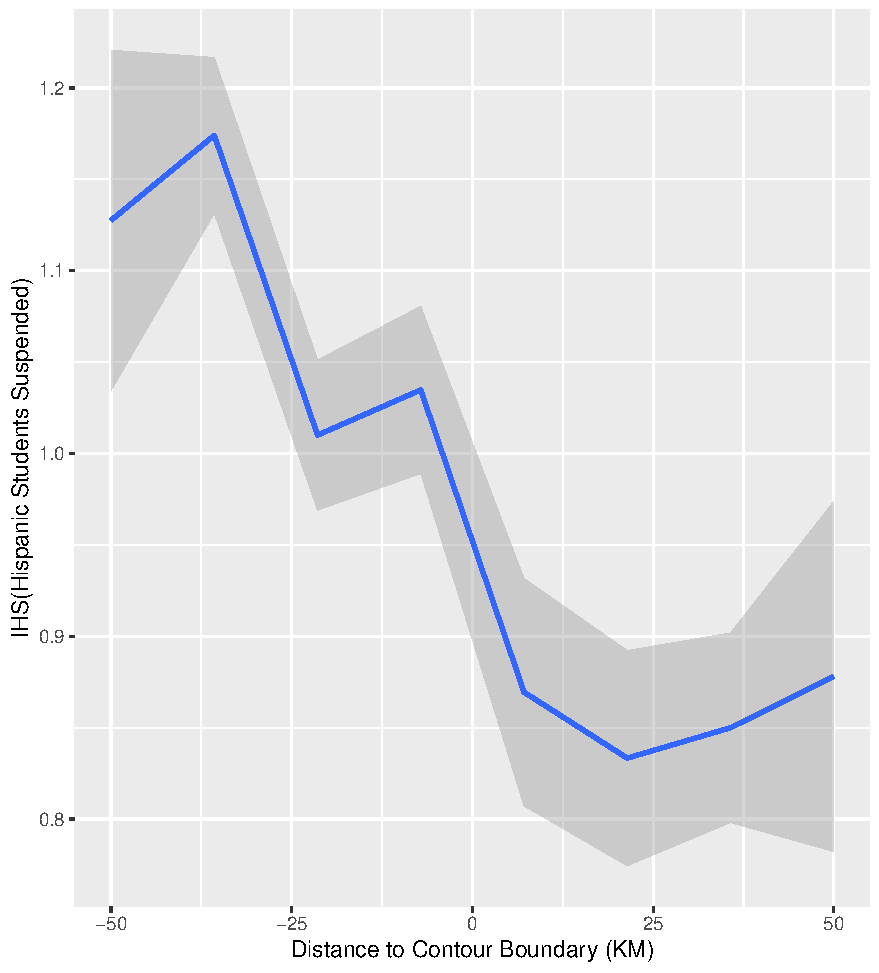
\includegraphics[width=12cm]{../../analysis/Output/graphs/hispanicsuspensions.pdf}
%
%\textit{Notes:} The figure presents data at a school level, where a smoothed average of the inverse hyperbolic sine transformed counts of Hispanic students suspended is plotted against the distance of the school to the closest Spanish Language Television station contour boundary. Positive distances denote schools that are located within the boundary, while negative distances denote schools outside of them.
%\end{figure} 



%\begin{figure}[!hbtp]
%\centering
%\caption{Coverage map for TV station WUVC-DT}\label{f:contour_example}
%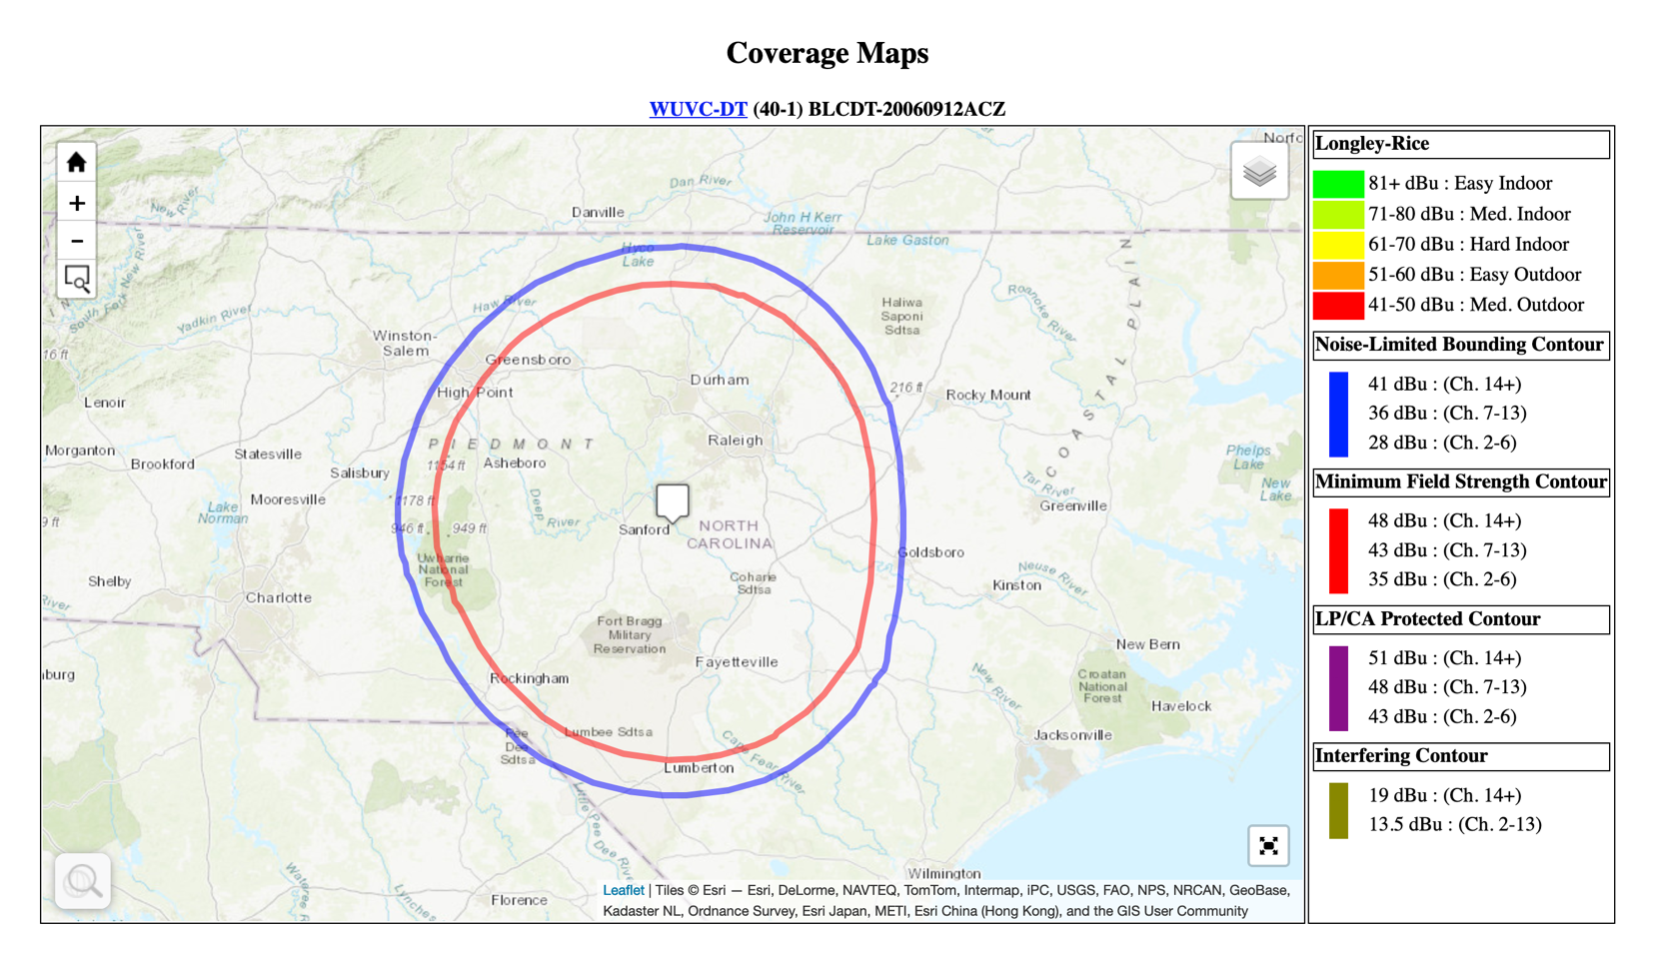
\includegraphics[width=6cm]{../../analysis/Output/img/ContourExample.png}
%\end{figure} 
%
%\begin{figure}[!hbtp]
%\centering
%\caption{Map of coverage contours of Spanish Language TV stations and public schools in the US}\label{f:contours_schools}
%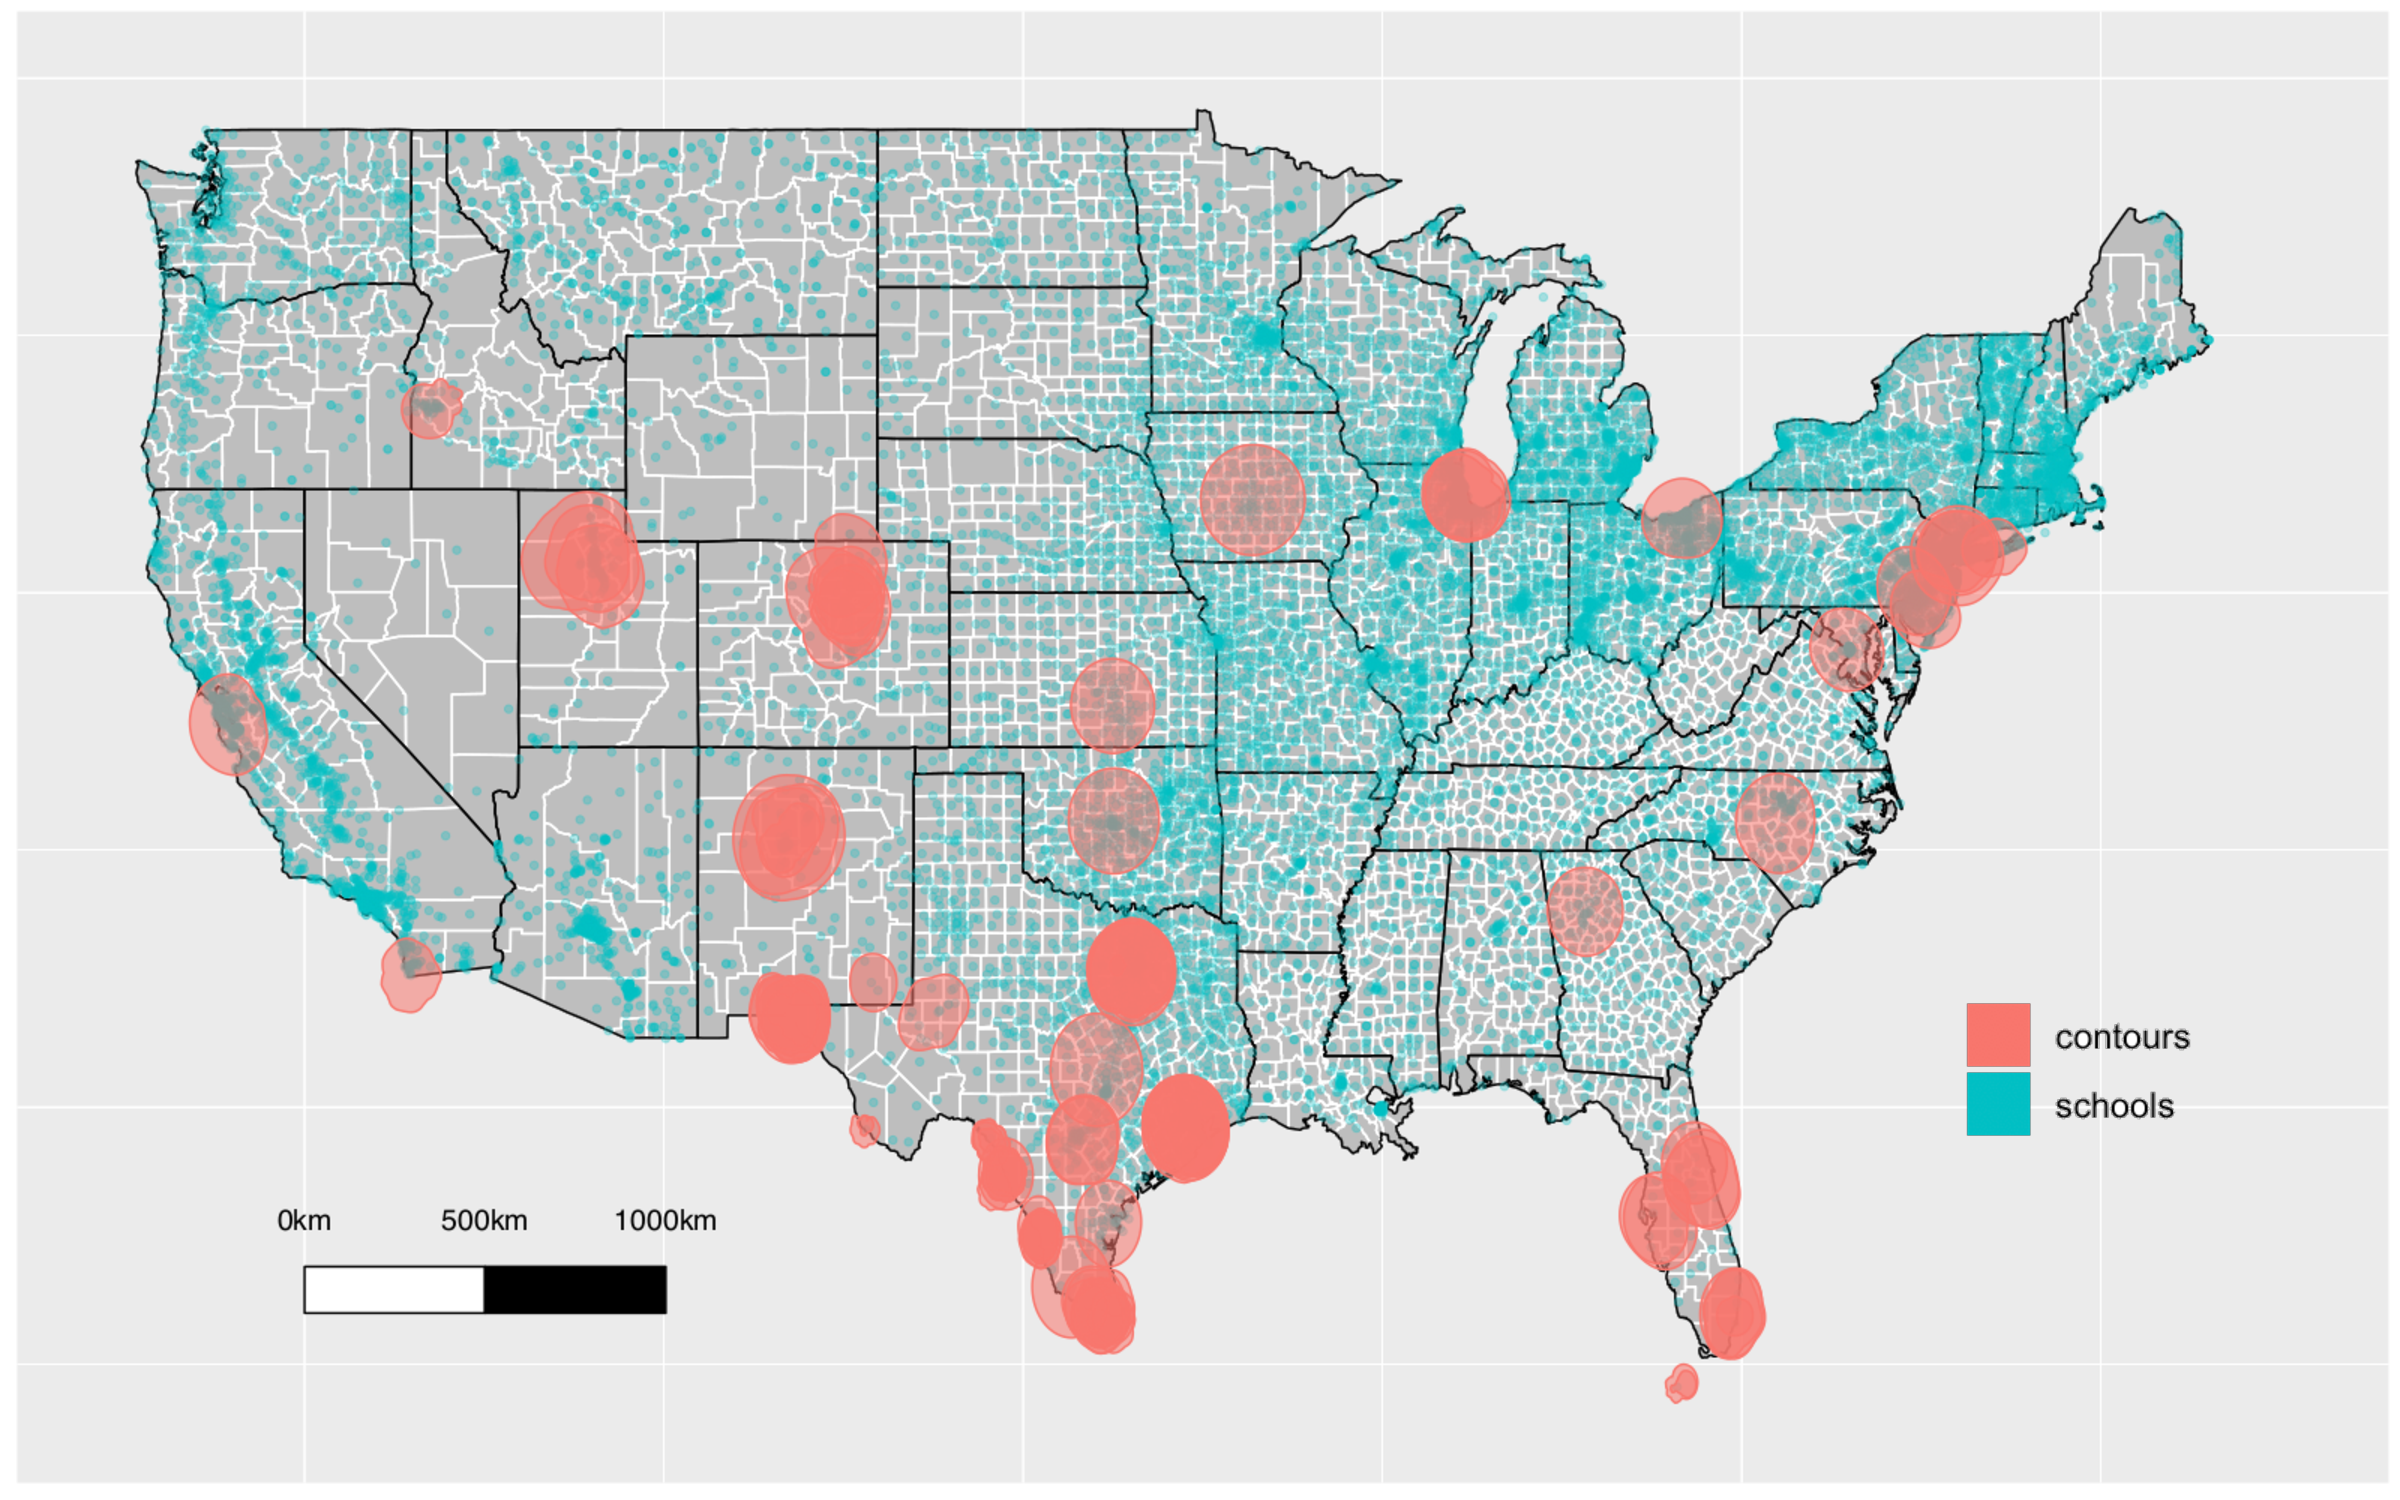
\includegraphics[width=6cm]{../../analysis/Output/img/Schools_pretty2.pdf}
%\end{figure} 

\begin{figure}[!hbtp]
\centering
\caption{Minutes of TV watched across the coverage contour}\label{f:atus}
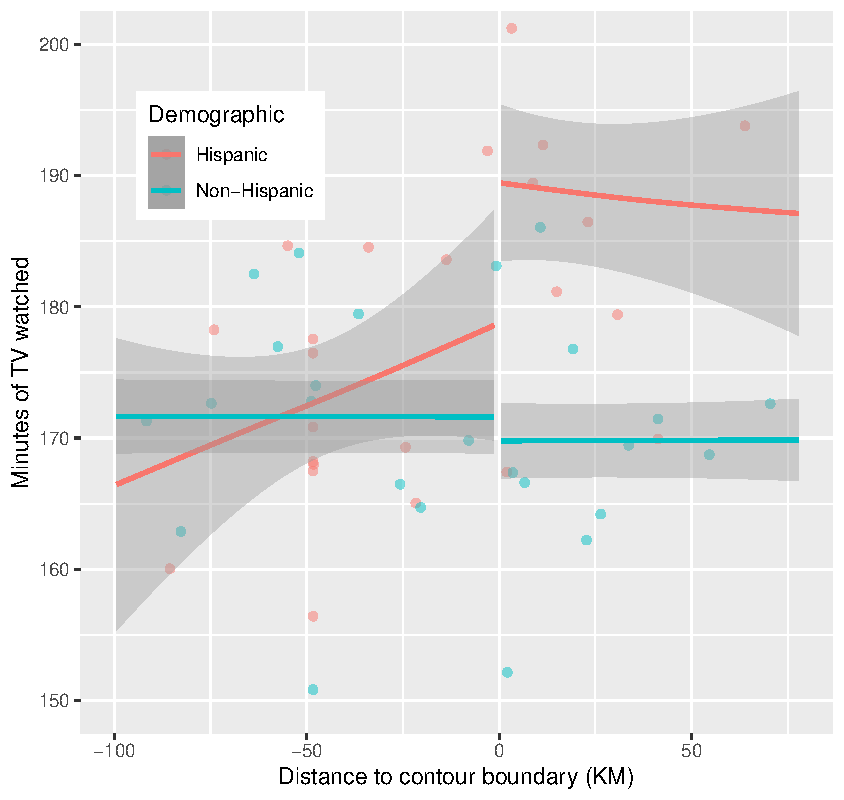
\includegraphics[width=14cm]{../../analysis/Output/graphs/atus2.pdf}
\caption*{Lowess smoothed (lines) and binscattered (points) minutes of television watched by distance to SLTV coverage contour boundary. Negative values indicate individuals outside of a contour (no SLTV). Hispanic viewership is in red, non-Hispanic viewership is in blue. Minutes of TV watched are residualized by individual level age, age$^2$, sex, and county level controls for log(income), log(population) and percent Hispanic. }
\end{figure} 


\clearpage

%\subsection{Tables}
%
%Table plan:
%\begin{enumerate}
%\item $<X>$ Summary stats table: ATUS data, education (school level), transcript data, Safegraph data
%\item $<X>$ ATUS: first stage (93), children (99), ATUS: parents (97),
%\item $<X>$ Education: top performance: gifted, SAT/ACT, AP passed, 
%\item $<X> $Education: identity
%\item $<X>$ Transcript: identity
%\item $<X>$ Safegraph: identity
%\end{enumerate}
%
%Appendix:
%\begin{enumerate}
%\item Migration table
%\item $<X>$ foreign born (94)
%\item Education: robustness
%\item Education: robustness spatial (SAR lag, SAR error)
%\item $<X>$ Education: more top performance
%\item Education: bottom performance?
%\item Transcript: bad identity
%\item Additional robustness
%\end{enumerate}

%\expandableinput{../../analysis/Output/regs/summary_main.tex}
%\expandableinput{../../analysis/Output/regs/atus_main.tex}
\expandableinput{../../analysis/Output/regs/edu_combine.tex}
\expandableinput{../../analysis/Output/regs/transcript_main.tex}
%\expandableinput{../../analysis/Output/regs/safegraph_main.tex}



\clearpage
\begin{singlespace}
\begin{scriptsize}
\bibliographystyle{aea}
%\bibliographystyle{plainnat}
\bibliography{tv}{}
\end{scriptsize}
\end{singlespace}

\pagebreak
\clearpage

%%%%%%%%%%%%%%%%%%%%%%
%%%%%%%%%%%%%%%%%%%%%%

%ONLINE APPENDIX MATERIAL


\clearpage

\singlespacing

\setcounter{footnote}{0}

\setcounter{section}{0}

\setcounter{page}{1}
\renewcommand\thepage{A.\arabic{page}}

\renewcommand*{\theHsection}{\arabic{section}.\arabic{section}} 

\renewcommand*{\theHfigure}{\arabic{section}.\arabic{figure}} 
\setcounter{figure}{0}
\renewcommand\thefigure{A.\arabic{figure}}


\renewcommand*{\theHtable}{\arabic{section}.\arabic{table}} 
\setcounter{table}{0}
\renewcommand\thetable{A.\arabic{table}}

\renewcommand{\thesection}{Appendix \Alph{section}}

\onehalfspacing

\begin{center}
\Large ONLINE APPENDIX
\end{center}

\section{Auxiliary data information} \label{a:auxiliarydata}

% In addition to the primary data sources described in Section~\ref{s:data}, we also use a number of auxiliary data sources for the empirical analysis.


\paragraph{Migration data}

Data on migration comes from the 2011-2015 American Community Survey (ACS), which reports the number of people moving from each origin county to destination county (aggregated over the five years).\footnote{ Historically, approximately 15\% of the ACS migration data has been allocated, or imputed based on salient characteristics (United States Census Bureau \cite{noauthor_american_2020}).} This sample also contains migration flows for the Hispanic population.

The migration data from the ACS is provided at the origin county-destination county level. I define a county as receiving SLTV if at least 50\% of the area that the county encompasses is inside of the coverage contour.\footnote{ Results are robust to different area cutoffs for a county to be considered inside the coverage contour.} There are 636 such counties (destination within 100 KM). The average origin county has 20 destination counties for which there is significant enough cross-county Hispanic migration that the ACS reports data for it.


% \paragraph{American Time Use (ATUS)} TV item code? Definition of parent/child?


\paragraph{Civil Rights Data Collection (CRDC)}

Below are descriptions of the academic outcomes as defined by the CRDC:
\begin{itemize}
\item \textbf{SAT/ACTs taken:}  The SAT Reasoning test ``is a nationally recognized assessment used to indicate college readiness. The SAT (formerly the Scholastic Aptitude Test) is sponsored by the College Board.''  The ACT test ``is a nationally recognized assessment used to indicate college readiness. The ACT is sponsored by ACT, Inc.'' (CRDC\cite{noauthor_master_2016}) Scores for one of the two exams were almost universally required for admission to colleges in the United States in 2015.

\item \textbf{Calculus taken:}  Calculus ``is a (college-preparatory) course with topics that include the study of derivatives, differentiation, integration, the definite and indefinite integral, and applications of calculus. Typically, students have previously attained knowledge of precalculus topics (some combination of trigonometry, elementary functions, analytic geometry, and math analysis).'' (CRDC\cite{noauthor_master_2016}) It is frequently the most advanced mathematics course offered in US high schools.


\item \textbf{AP programs passed:} %We focus on two outcomes that track the effect of television on the top end of the academic distribution of students: the number of Advanced Placement (AP) classes students enroll in and pass, as well as the number of students placed into gifted programs, and one outcome on the bottom: the number of students with Limited English Proficiency (LEP).
The AP program is administered by the College Board, and defines a standardized college-level curriculum that is taught to high school students in AP Classes. In conjunction with AP Classes, AP Exams are national examinations which are designed to test mastery of material taught in AP classes. These exams are scored on a scale ranging from 1 to 5, with scores below a 3 marked as a failed exam. Even among the students who select into these classes (22\% in 2015\footnote{ Data computed from number of high school graduates in 2015 (National Student Clearinghouse Research Center,\cite{noauthor_high_2015}), and number of seniors who sat an AP exam in 2015. This is how the College Board currently tracks national AP participation (no comparable summary statistic was released in 2015) (College Board,\cite{noauthor_ap_2015})}), a substantial number of students who take these exams fail them - approximately 35\% (College Board\cite{noauthor_ap_2020}). 

% \item \textbf{Gifted program enrollment:}  Gifted and talented programs are ``programs during regular school hours that provide special educational opportunities including accelerated promotion through grades and classes and an enriched curriculum for students who are endowed with a high degree of mental ability or who demonstrate unusual physical coordination, creativity, interest, or talent." (CRDC\cite{noauthor_master_2016}) These programs, while not mandatory, are common across school districts, and vary in their implementation. % HOW MANY STUDENTS?

\item \textbf{Limited English Proficiency (LEP):} LEP students (also called English Learner students) are students that, as a result of their limited command over the English language, have difficulty participating in regular school activities.\footnote{The specific definition of a LEP student depends on individual state regulation, but must also satisfy the criteria outlined under Title IX of the Elementary and Secondary Education Act). The most salient features of Title IX are that students must either not speak English as a native language or come from an environment where non-English languages are dominant, and also face substantial difficulty in engaging with others on the basis of their English ability.} 9\% of all public school students are considered LEP, and while students are placed into the program is at the discretion of individual school districts, all districts must provide language assistance services and have staff qualified to implement the LEP programs.\footnote{ Department of Justice and Department of Education,``Ensuring English Learner Students Can Participate Meaningfully and Equally in Educational Programs'' contains a full enumeration of the responsibilities school districts have. It further includes requirements such as ensuring equal access to various school programs etc. } 

\item \textbf{Ethnicity-based bullying:} Harassment or bullying on the basis of race, color, or national origin ``refers to intimidation or abusive behavior toward a student based on actual or perceived race, color, or national origin. Harassing conduct may take many forms, including verbal acts and name-calling, as well as non-verbal behavior, such as graphic and written statements, or conduct that is physically threatening, harmful or humiliating. The conduct can be carried out by school employees, other students, and non-employee third parties. Bullying on the basis of race, color, or national origin constitutes racial harassment." (CRDC,\cite{noauthor_master_2016}) A similar definition exists for bullying based on sex.

\end{itemize}

These variables are all reported at demographic level within schools. Additional outcomes used from the CRDC include the number of gifted students enrolled in the school, the number of students taking advanced math courses (including trigonometry, analytic geometry, math analysis, probability and statistics, and precalculus), enrollment in college preparatory courses for biology, physics, and chemistry, the number of students retained from one year to the next, and the number of students classified under IDEA (served under the Individuals with Disabilities Education Act). Additional variables from the CRDC used in the analysis include the address of the school (for geocoding), the school district, the number of total, Hispanic, and Asian students, and indicators for whether the school contains a primary school, middle school, and high school. School non-compliance on reporting for mandatory data typically represents $<1\%$ of total data.


% sample problems
% \footnote{ In practice, this data is not released to the public every year. Furthermore, not all schools report all data (or correct data) required of them, which is why the number of observations for different variables in this dataset fluctuates. Some data, such as that on AP examinations, are not mandatory, but the bulk of outcome variables are, with non-compliance on the mandatory data typically representing $<1\%$ of total data.} 

% TODO: propagate errors based on the margin of error


\paragraph{archive.org transcript data} 
Appendix Table~\ref{t:transcript_keywords} presents the keywords within SLTV transcripts used to identify each mechanism.  Panel A contains the list of word stubs for Hispanic countries. Given that about half of all SLTV programming is locally produced or translations of US television content (such as news, the weather, or sports), these keywords are meant to capture the SLTV programming that is either produced abroad or focused on events abroad. Panel B contains a list of common words relating to education. This is meant to capture the extent to which a TV program focuses on education. Panel C contains a list of telenovelas (television dramas) aimed at children with good role models that aired before 2015. 

Data is collected at the parent network level and values for each network is assigned to each affiliate TV station. Transcript data from the parent network is a reasonable proxy for local television content given that more than half the content in SLTV stations are either sourced internationally or produced for national consumption. 

\paragraph{Safegraph foot-traffic data} 
Restaurants in the Safegraph data are tagged with the kind of cuisine that they serve. I classify a restaurant as Hispanic-branded if any of the following tags apply to it: `Argentinean Food', `Cuban Food', `Latin American Food', `Mexican Food', `Peruvian Food', `Spanish Food', `Tapas'. `Japanese Food', `Brazilian Food', and `Cajun and Creole Food' are the tags used for the respective branding.

Other non-restaurant establishments do not contain explicit tags (relating to nationality or otherwise). Thus, for internal consistency, I classify recreation establishments using the same keyword matching procedure as the TV transcript data. The same set of countries used for identity-based SLTV transcripts are used to identify Hispanic-branded establishments. For Japan and Brazil, these country name stubs are used. For the case of Cajun and Creole, the case-insensitive terms `cajun', `creole', `haiti', and `jamaica' are used (the latter two representing the two largest countries with substantial Creole speaking populations). A manual check of 100 restaurants and recreation establishments validates that these locations are correctly classified.

% TODO: talk about imputing process for CBG and Heckman correction


\paragraph{Geocoding}

Geocoding based on address names is performed by ArcGIS to obtain a particular latitude/longitude. The US Census Geocoder is used to validate these locations. This geocoding procedure is successful over 99.9\% of the time. Schools and other locations not successfully geocoded are dropped from the sample. For counties and other non-point locations, distances to the SLTV coverage contour boundary are computed using the minimum distance from the region to the boundary.


\clearpage

\section{Hispanic migration across SLTV boundaries}\label{a:migration}

One concern for identification is that Hispanics may move based on access to SLTV, causing results to be driven by selection. I investigate whether this occurs using census data on migration. As mentioned in \ref{a:auxiliarydata}, this migration data is provided at the origin county-destination county level. Given the relative size of a county, I define a county as receiving SLTV if at least 50\% of its area is inside of the SLTV coverage contour.\footnote{ Results are robust to different area cutoffs for a county to be considered inside the coverage contour.} I present summary statistics for this sample in Table \ref{t:summary_migration}.

Given the role that the distance between counties plays in migration distances, I modify the difference-in-discontinuities approach to this interaction. The main specification is also adapted slightly for this data at the origin county-destination county-ethnicity level. The first specification I examine is:

\[ y_{o,d,j} =  \beta \mathbb{I}[InsideContour_{o}] \times \mathbb{I}[Hispanic_{j}] \times Distance_{o,d} + \gamma_d + \delta  X_o + \epsilon_{o,d,j} \]

where $o$ indexes an origin county, $d$ a destination county, and $j$ is a demographic category (Hispanic or not). This first specification only keeps destination counties that are within 100 KM of the contour boundary. To test for whether Hispanics differentially cross the contour boundary when moving, I split the sample into destination counties inside \& outside the contour and test for whether they differentially migrate to contours outside or into the contour respectively: therefore, the coefficient of interest is the interaction between $InsideContour_o$ and $Hispanic$ indicator. All specifications include destination fixed effects and controls at the origin county level.

Table \ref{t:mig_dd_dest} presents this regression, where the outcome is the inverse hyperbolic sine transformed value of the number of migrants between the two counties. Panel A shows the sample where destination counties are inside the contour and finds that Hispanics do not differentially migrate to counties outside the contour. Panel B shows the sample where destination counties are outside the contour and finds that Hispanics do not differentially migrate to counties inside the contour. Coefficients are stable across columns, which add origin county level controls for log(population), \% county Hispanic, and mean log(income) in each successive column.

Table  \ref{t:mig_dd_orig} changes the sample to those where the origin county are within 100 KM of the contour boundary. This specification flips the $o,d$ subscripts, so that the specification is now: 

\[ y_{o,d,j} =  \beta \mathbb{I}[InsideContour_{d}] \times \mathbb{I}[Hispanic_{j}] \times Distance_{o,d} + \gamma_o + \delta  X_d + \epsilon_{o,d,j} \]

which can be interpreted similarly, except that we are now looking at migration to a given destination county conditional on viewing their origin county. Table \ref{t:mig_dd_orig}, Panel A shows the sample where origin counties are inside the contour and finds that Hispanics do not migrate in greater numbers across the contour. Panel B shows the sample where origin counties are outside the contour and finds that Hispanics do not differentially migrate in greater numbers across the contour. In fact, these results show a negative sign, suggesting that if anything, Hispanics are averse to moving across these boundaries. This is sufficient for me to make the argument that there is no selection, given that so long as there are not positive coefficients, there is no evidence of migration across contour borders.\footnote{ One potential reason for aversion to moving across the contour boundary could be the tightness of Hispanic communities with SLTV if there is indeed an identity mechanism at play, or simply something in common to bond over.} One might wonder why results are not symmetric to those displayed in Table \ref{t:mig_dd_dest}. This is due to the census data censoring counties for which there is a low number of migrants. 

Tables \ref{t:mig_dest} and \ref{t:mig_orig} replicate the prior analysis, but now uses only the regression discontinuity interacted with the Hispanic indicator, and so no longer examines the differential amount of migration, but rather the absolute. The null result remains when examining the destination sample and, reassuringly, it does too in the origin sample as well too. 

But even in cases where significant results are observed, the base rate of migration is sufficiently low that it should not drive results. in the origin county sample, an average of 84 Hispanic people are observed to move between each county-county pair (median: 25) over the five year period which the dataset spans. This also speaks to the magnitude of the coefficients observed, where the drop in 10 to 40\% of migrants observed is plausible if it induces slightly fewer people to move. 

These results combined indicate that movement across coverage contours is not a major threat to identification. 


\clearpage

\section{Additional figures and tables}

\begin{figure}[!hbtp]
\centering
\caption{Map of coverage contours of Spanish Language TV stations and public schools within 100 KM of the contour boundary in the US}\label{f:contours_schools_inside}
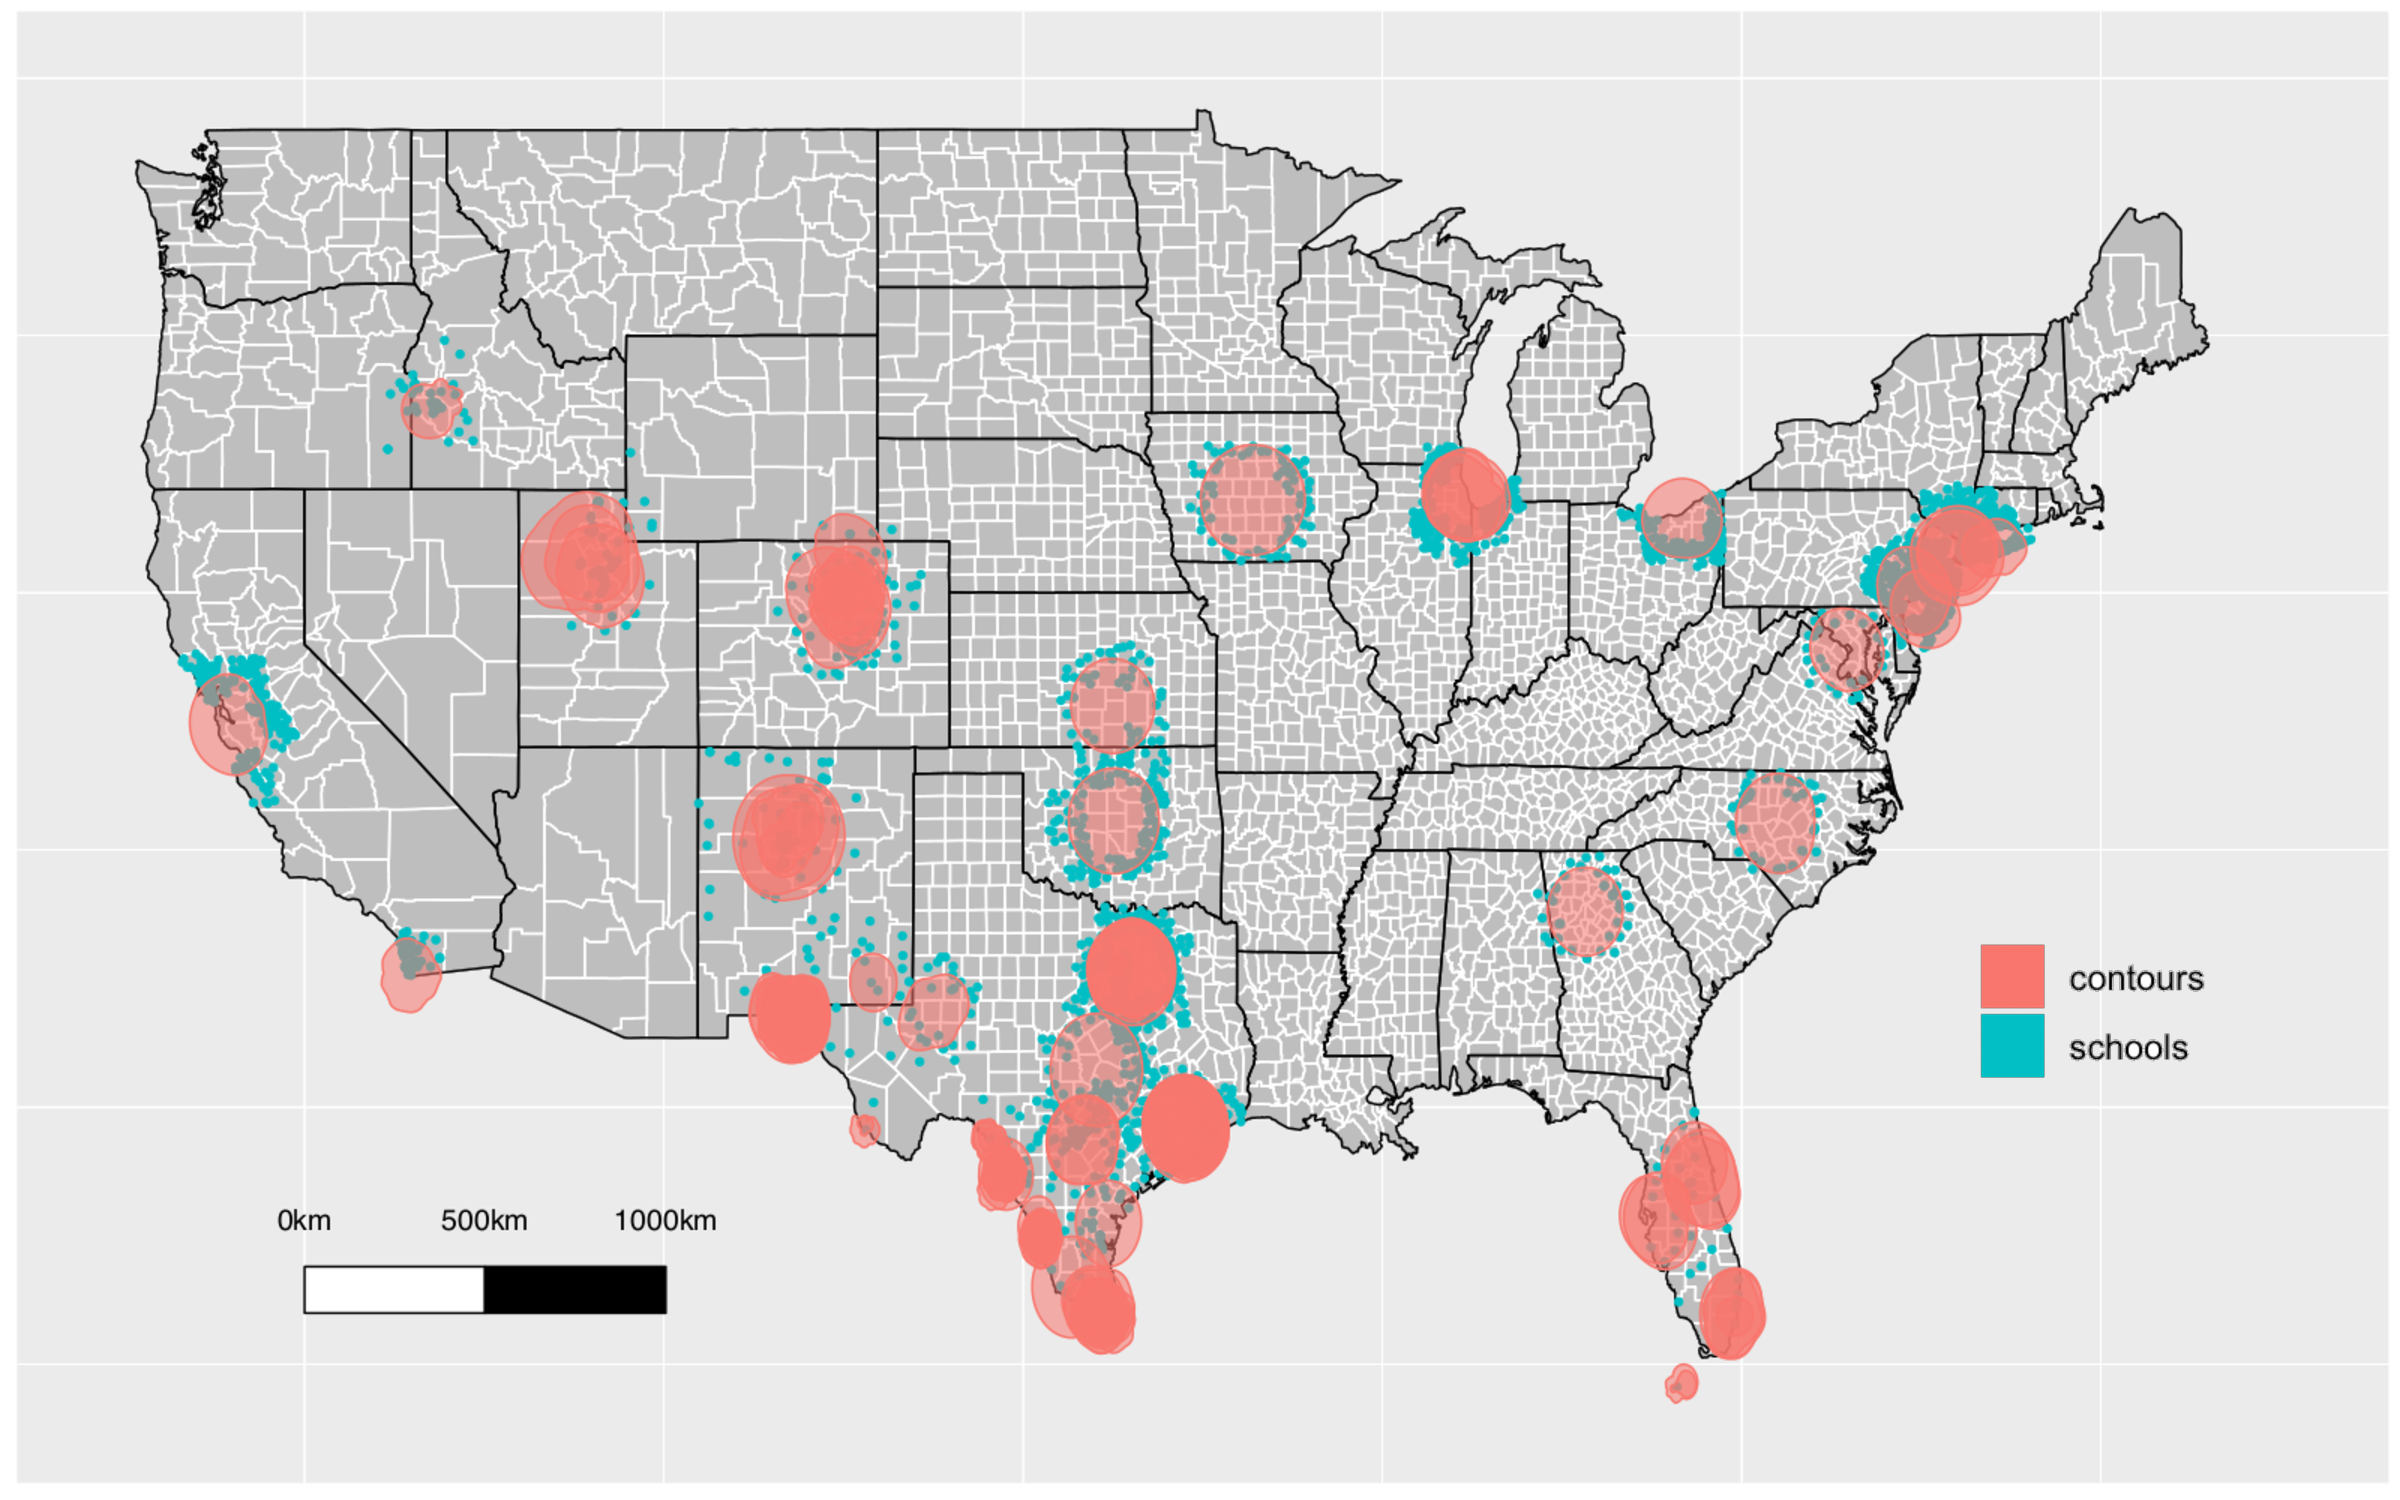
\includegraphics[width=14.4cm]{../../analysis/Output/img/Schools_inside2.pdf}
\end{figure} 

% TODO: map contours by parent network?
% TODO: map all POIs
% TODO: results by gender

% TODO: ATUS, where decrease in time?
% TODO: ATUS vs Asian
% TODO: (future) safegraph vs. Asian
% TODO: safegraph brand (chain) vs. no brand


\clearpage
\begin{table}[!h]
	\centering
	\captionsetup{skip=1.5pt}
	\caption{TV transcript keywords} \label{t:transcript_keywords}
	\scalebox{.8}{
	 	\begin{threeparttable}
			\begin{tabular}{llcccccccc}
				\hline\hline\addlinespace
    \textit{Panel A: Hispanic references} & mexic, bolivia, chile, argentin, venezuela, beliz, costa rica, salvador, guatemala \\
&  hondur, nicaragua, panama, colombia, ecuador, guyana, paragua, peru \\
& urugu, cuba, dominican, puerto, latin \\
				\addlinespace\hline
\textit{Panel B: Education references} &educación , enseñanza, colegio, escuela, universidad, estudio, estudiar, estudiante\\  
& alumna, alumno, profesora, profesor, maestro, maestra, clase, rango, grado \\
& aprender, mates, matematicas \\
\hline
\textit{Panel C: Role model references} & Vivan los niños, Alegrijes y rebujos, Aventuras en El tiempo, amigos por siempre \\
					& Misión S.O.S., Carrusel y El abuelo y Yo, El Juego de la Vida, De pocas pulgas\\
					& luz Clarita, Serafín, 31 minutos, Bizbirije, Odisea Burbujas, El Tesoro del Saber \\
					& Topo Gigio, Once Niñas y Niños \\		 		
				\addlinespace\hline\hline
			\end{tabular}
			\begin{tablenotes}[flushleft]
				\item \textit{Notes:} Television transcripts are classified as containing a reference name if any keyword (or program title in Panel C) in the panel is exactly matched within the word, ignoring case. Panel A contains the list of word stubs for Hispanic countries. Panel B contains a list of common words relating to education. Panel C contains a list of telenovelas with good role models for children that aired before 2015.
			\end{tablenotes}
		\end{threeparttable}
	}
\end{table}

\expandableinput{../../analysis/Output/regs/atus_foreign.tex}

\expandableinput{../../analysis/Output/regs/edu_magnitude.tex}
\expandableinput{../../analysis/Output/regs/edu_abs.tex}
\expandableinput{../../analysis/Output/regs/edu_extra_achieve.tex}
\clearpage
\expandableinput{../../analysis/Output/regs/edu_robust.tex}
\clearpage
\expandableinput{../../analysis/Output/regs/edu_retain.tex}

\expandableinput{../../analysis/Output/regs/edu_mech_placebo.tex}
\expandableinput{../../analysis/Output/regs/edu_mech_abs.tex}

\expandableinput{../../analysis/Output/regs/transcript_abs.tex}
\expandableinput{../../analysis/Output/regs/atus_edu.tex}

\expandableinput{../../analysis/Output/regs/safegraph_abs.tex}

\begin{table}[!h]
	\centering
	\captionsetup{skip=1.5pt}
	\caption{Summary statistics --- migration}\label{t:summary_migration}
	\scalebox{.8}{
		\begin{threeparttable}
			\begin{tabular}{l@{\extracolsep{4pt}}cccc}
				\hline\hline\addlinespace
				& \textit{All} &  \textit{No SLTV} & \textit{SLTV} \\
				\cline{2-4} \addlinespace
				& (1) & (2) & (3) \\
				\hline\addlinespace
				 \multicolumn{4}{l}{Panel A: Census migration data (county-county level) } \\
				\hline\addlinespace
				Origin county, IHS(Hispanic Migrants) & 4.391 & 4.548 & 4.086 \\
				& (1.281) & (1.336) & (1.104) \\
				Destination county, IHS(Hispanic Migrants) & 4.012 & 3.992 & 4.038 \\
				& (1.201) & (1.252) & (1.132) \\
				Observations & 12,551 & 12,551 & 12,551 \\
				\hline\addlinespace
				 \hline\addlinespace
			\end{tabular}
			\begin{tablenotes}[flushleft]
				\item \textit{Notes:} The table presents means (and standard deviations). Variables in Panel A are data from counties within 100 KM of a coverage contour. Columns 2 and 3 show data for the subsample without and with SLTV coverage, respectively. 
			\end{tablenotes}
		\end{threeparttable}
	}
\end{table}

\clearpage
\begin{table}[!h]
	\centering
	\captionsetup{skip=1.5pt}
	\caption{Effect of Spanish Language TV on Hispanic vs. non-Hispanic migration between counties --- destination sample} \label{t:mig_dd_dest}
	\scalebox{.8}{
		\begin{threeparttable}
			\begin{tabular}{lcccccccccc}
				\hline\hline\addlinespace
				& \multicolumn{3}{c}{IHS(\# Migrants)} \\
				\cline{2-4} 
				&  (1) & (2) & (3) \\
                                \hline\addlinespace
				\multicolumn{4}{l}{Panel A: Destination county inside contour} \\ %mig_odd_cl.tex
                                \hline\addlinespace
Origin outside TV contour $\times$ Hispanic &   0.0445 & 0.0446 & 0.0430\\
  &(0.2055) & (0.2057) & (0.2060)\\
  \addlinespace\hline\addlinespace
Observations & 21,826&21,826&21,826 \\
\hline\addlinespace
\multicolumn{4}{l}{Panel B: Destination county outside contour} \\  %migrev_odd_cl.tex
\hline\addlinespace
Origin inside TV contour $\times$ Hispanic & 0.0056 & 0.0049 & 0.0072\\
  &(0.2786) & (0.2794) & (0.2798)\\
 \addlinespace \hline\addlinespace
Observations & 11,098 & 11,098 & 11,098 \\        
\hline\addlinespace
                                Destination F.E. & Yes & Yes  & Yes\\
                                Distance, distance $^2$ & Yes & Yes & Yes \\
                                Origin log(pop.) & Yes & Yes & Yes \\
                                Origin \% Hispanic & No & Yes & Yes \\
                                Origin log(income) & No & No & Yes \\
				\addlinespace\hline\hline
			\end{tabular}
			\begin{tablenotes}[flushleft]
				\item \textit{Notes:} The table presents coefficient estimates from regressions at the origin county-destination county-ethnicity level, only keeping destination counties within 100 KM of a contour boundary. The dependent variables are inverse hyperbolic sine transformed counts of migrants from the origin county to the destination county. The key dependent variable of interest is an indicator for whether the origin county has access to SLTV interacted with a Hispanic indicator (the omitted group is non-Hispanic). This is interacted with the distance and distance-squared to the boundary for both the origin and destination county. Columns 1-3 include individual demographic controls for sex, age, and age squared, as well as the mean log(income) of the county. Columns 2-3 control for the percentage of the county that is Hispanic. Column 3 controls for the county's log(population). All regressions also contain destination county fixed effects. Standard errors are two-way clustered by origin and destination county. *, **, and *** denote statistical significance at the 10\%, 5\%, and 1\% levels, respectively.
			\end{tablenotes}
		\end{threeparttable}
	}
\end{table}
\begin{table}[!h]
	\centering
	\captionsetup{skip=1.5pt}
	\caption{Effect of Spanish Language TV on Hispanic vs. non-Hispanic migration between counties --- origin sample} \label{t:mig_dd_orig}
	\scalebox{.8}{
		\begin{threeparttable}
			\begin{tabular}{lcccccccccc}
				\hline\hline\addlinespace
				& \multicolumn{3}{c}{IHS(\# Migrants)} \\
				\cline{2-4} 
				&  (1) & (2) & (3) \\
                                \hline\addlinespace
				\multicolumn{4}{l}{Panel A: Origin county inside contour} \\
                                \hline\addlinespace
Destination outside TV contour $\times$ Hispanic &  -0.1225$^{**}$ & -0.1205$^{**}$ & -0.1210$^{**}$\\
  &(0.0541) & (0.0536) & (0.0537)\\ 
   \addlinespace\hline\addlinespace
Observations & 36,060&36,060&36,060 \\
\hline\addlinespace
\multicolumn{4}{l}{Panel B: Origin county outside contour} \\ 
\hline\addlinespace
Destination inside TV contour $\times$ Hispanic &  -0.1679$^{**}$ & -0.1679$^{**}$ & -0.1682$^{**}$\\
  &(0.0828) & (0.0828) & (0.0828)\\
   \addlinespace \hline\addlinespace
Observations & 20,692 & 20,692 & 20,692 \\        
\hline\addlinespace
                                Origin F.E. & Yes & Yes  & Yes\\
                                Distance, distance $^2$ & Yes & Yes & Yes \\
                                Distance log(pop.) & Yes & Yes & Yes \\
                                Distance \% Hispanic & No & Yes & Yes \\
                                Distance log(income) & No & No & Yes \\
				\addlinespace\hline\hline
			\end{tabular}
			\begin{tablenotes}[flushleft]
				\item \textit{Notes:} The table presents coefficient estimates from regressions at the origin county-destination county-ethnicity level, only keeping origin counties within 100 KM of a contour boundary. The dependent variables are inverse hyperbolic sine transformed counts of migrants from the origin county to the destination county. The key dependent variable of interest is an indicator for whether the destination county has access to SLTV interacted with a Hispanic indicator (the omitted group is non-Hispanic). This is interacted with the distance and distance-squared to the boundary for both the origin and destination county. Columns 1-3 include individual demographic controls for sex, age, and age squared, as well as the mean log(income) of the county. Columns 2-3 control for the percentage of the county that is Hispanic. Column 3 controls for the county's log(population). All regressions also contain origin county fixed effects. Standard errors are two-way clustered by origin and destination county. *, **, and *** denote statistical significance at the 10\%, 5\%, and 1\% levels, respectively.
			\end{tablenotes}
		\end{threeparttable}
	}
\end{table}
\begin{table}[!h]
	\centering
	\captionsetup{skip=1.5pt}
	\caption{Influence of Spanish Language Television on Migration Between Counties - Destination Sample} \label{mig_dest}
	\scalebox{.7}{
		\begin{threeparttable}
			\begin{tabular}{lcccccccccc}
				\hline\hline\addlinespace
				& \multicolumn{3}{c}{IHS(\# Hispanic Migrants)} \\
				\cline{2-4} 
				Panel A: Destination County Inside Contour&  (1) & (2) & (3) \\
                                \hline\addlinespace
 Dummy: Origin Outside TV Contour & $-$0.410$^{***}$ & $-$0.356$^{***}$ & $-$0.349$^{***}$ \\ 
  & (0.088) & (0.082) & (0.081) \\ 
 TV Dummy $\times$ Distance to Destination & $-$0.007$^{***}$ & $-$0.008$^{***}$ & $-$0.008$^{***}$ \\ 
  & (0.003) & (0.003) & (0.003) \\ 
 TV Dummy $\times$ Distance to Origin & $-$0.002 & $-$0.004$^{**}$ & $-$0.004$^{*}$ \\ 
  & (0.002) & (0.002) & (0.002) \\ 
 Distance from Contor to Destination (KM) & 0.002 & 0.004$^{**}$ & 0.004$^{**}$ \\ 
  & (0.002) & (0.002) & (0.002) \\ 
 Distance from Contour to Origin (KM) & 0.001 & 0.004 & 0.003 \\ 
  & (0.002) & (0.002) & (0.002) \\ 
 Destination Log(Population) & 0.179$^{***}$ & 0.181$^{***}$ & 0.175$^{***}$ \\ 
  & (0.019) & (0.016) & (0.019) \\ 
 Origin Log(Population) & 0.115$^{***}$ & 0.117$^{***}$ & 0.102$^{***}$ \\ 
  & (0.018) & (0.017) & (0.020) \\ 
 Destination \% Hispanic &  & 1.384$^{***}$ & 1.428$^{***}$ \\ 
  &  & (0.183) & (0.205) \\ 
 Origin \% Hispanic &  & 0.813$^{***}$ & 0.949$^{***}$ \\ 
  &  & (0.182) & (0.203) \\ 
 Destination Log(Income) &  &  & 0.041 \\ 
  &  &  & (0.099) \\ 
 Origin Log(Income) &  &  & 0.138 \\ 
  &  &  & (0.109) \\ 
Observations & 4,338 & 4,338 & 4,338 \\ 
\hline\addlinespace
Panel B: Origin County Outside Contour & & & \\ 
\hline\addlinespace
 Dummy: Origin Inside TV Contour & $-$0.140 & $-$0.194 & $-$0.193 \\ 
  & (0.152) & (0.144) & (0.144) \\ 
 TV Dummy $\times$ Distance to Destination & $-$0.004$^{*}$ & $-$0.007$^{***}$ & $-$0.007$^{***}$ \\ 
  & (0.002) & (0.002) & (0.002) \\ 
 TV Dummy $\times$ Distance to Origin & $-$0.007$^{**}$ & $-$0.004 & $-$0.004 \\ 
  & (0.003) & (0.003) & (0.003) \\ 
 Distance from Contor to Destination (KM) & $-$0.0003 & 0.002 & 0.002 \\ 
  & (0.002) & (0.001) & (0.001) \\ 
 Distance from Contour to Origin (KM) & $-$0.001$^{***}$ & $-$0.002$^{***}$ & $-$0.002$^{***}$ \\ 
  & (0.0004) & (0.0004) & (0.0004) \\ 
 Destination Log(Population) & 0.253$^{***}$ & 0.169$^{***}$ & 0.153$^{***}$ \\ 
  & (0.041) & (0.023) & (0.030) \\ 
 Origin Log(Population) & 0.182$^{***}$ & 0.181$^{***}$ & 0.181$^{***}$ \\ 
  & (0.035) & (0.030) & (0.034) \\ 
 Destination \% Hispanic &  & 2.324$^{***}$ & 2.471$^{***}$ \\ 
  &  & (0.389) & (0.411) \\ 
 Origin \% Hispanic &  & 1.276$^{**}$ & 1.253$^{**}$ \\ 
  &  & (0.602) & (0.584) \\ 
 Destination Log(Income) &  &  & 0.181 \\ 
  &  &  & (0.196) \\ 
 Origin Log(Income) &  &  & $-$0.015 \\ 
  &  &  & (0.192) \\ 
Observations & 1,659 & 1,659 & 1,659 \\        
\hline\addlinespace
                                Destination F.E. & Yes & Yes  & Yes\\
				\addlinespace\hline\hline
			\end{tabular}
			\begin{tablenotes}[flushleft]
				\item \textit{Notes:} The table presents coefficient estimates from regressions at the county-county level, only keeping destination counties within 100 KM of a contour boundary. The dependent variables are inverse hyperbolic sine transformed counts of Hispanic migrants from the origin county to the destination county. The key dependent variable of interest is the TV Dummy, which tracks whether the destination county is inside or outside the TV contour. This is interacted with the distance to the boundary for both the origin and destination county. County controls include log income, log population, and percentage county Hispanic for both origin and destination county. All regressions also contain destination county fixed effects. Standard errors are given in parentheses. *, **, and *** denote statistical significance at the 10\%, 5\%, and 1\% levels, respectively.
			\end{tablenotes}
		\end{threeparttable}
	}
\end{table}
\begin{table}[!h]
	\centering
	\captionsetup{skip=1.5pt}
	\caption{Influence of Spanish Language Television on Migration Between Counties - Origin Sample} \label{t:mig_orig}
	\scalebox{.7}{
		\begin{threeparttable}
			\begin{tabular}{lcccccccccc}
				\hline\hline\addlinespace
				& \multicolumn{3}{c}{IHS(\# Hispanic Migrants)} \\
				\cline{2-4} 
				Panel A: Origin County Inside Contour&  (1) & (2) & (3) \\
                                \hline\addlinespace
Dummy: Destination Outside TV Contour & $-$0.387$^{***}$ & $-$0.286$^{***}$ & $-$0.280$^{***}$ \\ 
  & (0.048) & (0.044) & (0.044) \\ 
 TV Dummy $\times$ Distance to Origin & $-$0.003$^{**}$ & $-$0.004$^{***}$ & $-$0.004$^{***}$ \\ 
  & (0.001) & (0.001) & (0.001) \\ 
 TV Dummy $\times$ Distance to Destination & 0.001 & $-$0.002$^{*}$ & $-$0.002 \\ 
  & (0.001) & (0.001) & (0.001) \\ 
 Distance from Contour to Origin (KM) & 0.001 & 0.003$^{*}$ & 0.003 \\ 
  & (0.002) & (0.002) & (0.002) \\ 
 Distance from Contour to Destination (KM) & $-$0.001 & 0.002 & 0.002 \\ 
  & (0.001) & (0.001) & (0.001) \\ 
 Origin Log(Population) & 0.146$^{***}$ & 0.161$^{***}$ & 0.150$^{***}$ \\ 
  & (0.020) & (0.017) & (0.021) \\ 
 Destination Log(Population) & 0.150$^{***}$ & 0.136$^{***}$ & 0.125$^{***}$ \\ 
  & (0.014) & (0.013) & (0.016) \\ 
 Origin \% Hispanic &  & 0.792$^{***}$ & 0.881$^{***}$ \\ 
  &  & (0.103) & (0.141) \\ 
 Destination \% Hispanic &  & 1.485$^{***}$ & 1.573$^{***}$ \\ 
  &  & (0.122) & (0.141) \\ 
 Origin Log(Income) &  &  & 0.093 \\ 
  &  &  & (0.094) \\ 
 Destination Log(Income) &  &  & 0.090 \\ 
  &  &  & (0.078) \\ 
Observations & 8,479 & 8,479 & 8,479 \\ 
\hline\addlinespace
Panel B: Origin County Outside Contour & & & \\ 
\hline\addlinespace
 Dummy: Destination Inside TV Contour & $-$0.078 & $-$0.123 & $-$0.120 \\ 
  & (0.108) & (0.096) & (0.096) \\ 
 TV Dummy $\times$ Distance to Origin & $-$0.003$^{*}$ & $-$0.004$^{***}$ & $-$0.004$^{***}$ \\ 
  & (0.002) & (0.001) & (0.001) \\ 
 TV Dummy $\times$ Distance to Destination & $-$0.004$^{***}$ & $-$0.002 & $-$0.002 \\ 
  & (0.001) & (0.001) & (0.001) \\ 
 Distance from Contour to Origin (KM) & $-$0.0003 & 0.001 & 0.001 \\ 
  & (0.001) & (0.001) & (0.001) \\ 
 Distance from Contour to Destination (KM) & $-$0.001$^{***}$ & $-$0.001$^{***}$ & $-$0.001$^{***}$ \\ 
  & (0.0002) & (0.0003) & (0.0003) \\ 
 Origin Log(Population) & 0.164$^{***}$ & 0.131$^{***}$ & 0.094$^{***}$ \\ 
  & (0.017) & (0.021) & (0.026) \\ 
 Destination Log(Population) & 0.150$^{***}$ & 0.128$^{***}$ & 0.125$^{***}$ \\ 
  & (0.023) & (0.020) & (0.021) \\ 
 Origin \% Hispanic &  & 1.328$^{***}$ & 1.611$^{***}$ \\ 
  &  & (0.295) & (0.329) \\ 
 Destination \% Hispanic &  & 1.485$^{***}$ & 1.481$^{***}$ \\ 
  &  & (0.293) & (0.318) \\ 
 Origin Log(Income) &  &  & 0.407$^{**}$ \\ 
  &  &  & (0.193) \\ 
 Destination Log(Income) &  &  & 0.003 \\ 
  &  &  & (0.087) \\ 
Observations & 4,062 & 4,062 & 4,062 \\         
\hline\addlinespace
                                Origin F.E. & Yes & Yes  & Yes\\
				\addlinespace\hline\hline
			\end{tabular}
			\begin{tablenotes}[flushleft]
				\item \textit{Notes:} The table presents coefficient estimates from regressions at the county-county level, only keeping origin counties within 100 KM of a contour boundary. The dependent variables are inverse hyperbolic sine transformed counts of Hispanic migrants from the origin county to the destination county. The key dependent variable of interest is the TV Dummy, which tracks whether the destination county is inside or outside the TV contour. This is interacted with the distance to the boundary for both the origin and destination county. County controls include log income, log population, and percentage county Hispanic for both origin and destination county. All regressions also contain origin county fixed effects. Standard errors are given in parentheses. *, **, and *** denote statistical significance at the 10\%, 5\%, and 1\% levels, respectively.
			\end{tablenotes}
		\end{threeparttable}
	}
\end{table}





\pagebreak




\end{document}


%Resources:
%https://rpubs.com/chrisbrunsdon/114718
%https://rpubs.com/corey_sparks/109650
%http://www.econ.uiuc.edu/~lab/workshop/Spatial_in_R.html
%https://rspatial.org/raster/analysis/7-spregression.html
%Conley Errors





 